\documentclass{article}
\usepackage{amsmath}
\usepackage{graphicx}
\usepackage{hyperref}

\title{Discrete Assignment}

\begin{document}

\section*{Discrete Assignment}
\textit{ee23btech11215,Penmetsa Srikar Varma,IC Design and Technology}
\subsection*{Question 10 of Exercise 5 of Chapter 9: Progressions and Series of class 11} 
\textbf{Q10)} The sum of three numbers in G.P. is 56. If we subtract 1, 7, 21 from these numbers in that order, we obtain an arithmetic progression. Find the numbers.\\\\
\textbf{Answer:}\\\\
Let us assume the first term of given geometric progression be $a(0)$ and common ratio be '\textit{r}'\\
\\Let the terms of \textit{GP} be:
$$a(0),a(1),a(2)...a(k)$$
From above we can say that $n^{th}$ term of \textit{GP} a(n) is given by:
\begin{equation}
\label{a1}
a(n)=a(0).r^n
\end{equation}
\textbf{Input table:}\\
\begin{center}
\begin{tabular}{|c|c|}
  \hline
    Input Variable & Input Condition \\
\hline
    $a(0)$ & first term of \text{GP} \\
\hline
    \textit{r} & common ratio of \textit{GP}\\
\hline
    $\frac{a(0)}{r},a(0),a(0).r$ & $\frac{a(0)}{r}+a(0)+a(0).r=56$ \\
\hline
    $\frac{a(0)}{r}-1,a(0)-7,a(0).r-21$ & form an \textit{AP}\\
\hline
\end{tabular}
\end{center}
We know that, if three numbers \textit{p},\textit{q} and \textit{r} are in arithmetic progression then,
\begin{equation}
\label{q1}
2q = p + r
\end{equation}
Let us assume three numbers which are in \textit{GP},
\[\frac{a(0)}{r},a(0),a(0).r\]
Then from given,
\[\frac{a(0)}{r}+a(0)+a(0).r=56\]
\[a(0).\left(\frac{1}{r}+1+r\right)=56\]
\begin{equation}
\label{q2}
a(0)=\frac{56}{\left(\frac{1}{r}+1+r\right)}
\end{equation}
and from given another case following are in \textit{AP},
\[\frac{a(0)}{r}-1,a(0)-7,a(0).r-21\]
Then from (\ref{q1}),
\[2.(a(0)-7)=\frac{a(0)}{r}-1+a(0).r-21\]
\[2.a(0)-14=\frac{a(0)}{r}+a(0).r-22\]
\[\frac{a(0)}{r}+a(0).r-2.a(0)=8\]
\[a(0)\left(\frac{1}{r}+r-2\right)=8\]
and from (\ref{q2})
\[\frac{56.\left(\frac{1}{r}+r-2\right)}{\left(\frac{1}{r}+1+r\right)}=8\]
\[7\left(\frac{1}{r}+r-2\right)=\left(\frac{1}{r}+1+r\right)\]
\[\frac{6}{r}+6.r-15=0\]
\[6.r^2-15.r+6=0=2.r^2-5.r+2\]
\[(2.r-1).(r-2)=0\]
\begin{equation}
\label{q3}
r=\frac{1}{2},2
\end{equation}
so from (\ref{q2}),
\[a(0)=16\]
Then from (\ref{a1}),
$$a(n)=16.2^n=2^{n+4}\quad for\ (r=2)\qquad and\qquad  a(n)=16.\left(\frac{1}{2}\right)^n=2^{4-n}\quad for\ (r=\frac{1}{2})$$
\begin{figure}
    \centering
    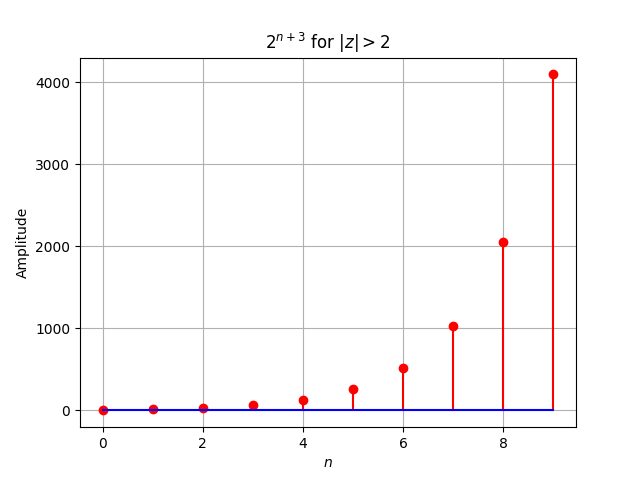
\includegraphics[scale=0.65]{py_1.png}
    %github/psrikarvarma/ss-assignment_1-jan2024/blob/main/discrete_sequences/figs/py_1.png}
    \caption{Graph of $2^{n+4}$}
    \label{fig:enter-label}
\end{figure}\\
\begin{figure}
    \centering
    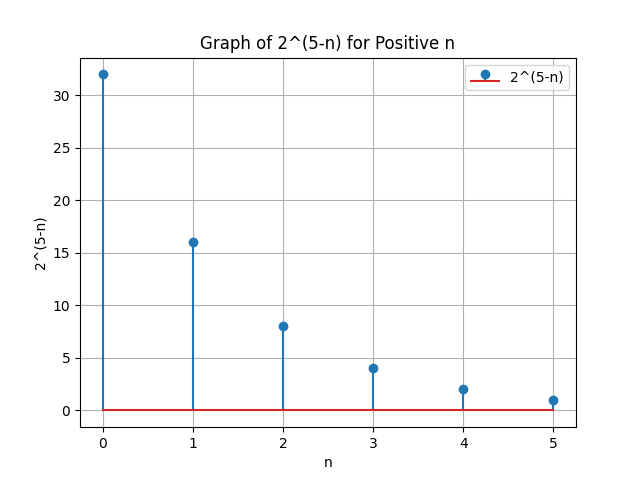
\includegraphics[scale=0.65]{py_2.png}
    %github/psrikarvarma/ss-assignment_1-jan2024/blob/main/discrete_sequences/figs/py_2.png}
    \caption{Graph of $2^{4-n}$}
    \label{fig:enter-label}
\end{figure}

\end{document}
